\documentclass[../main.tex]{subfiles}

\graphicspath{{../images/}}

\begin{document}
\pagestyle{fancy}
\lhead{Lecture 22: 11/14/24}
\chead{Chapter 7}
\rhead{PHYS 421}

\section{Electrodynamics}
\subsection{Electromotive Force}
\subsubsection{Ohm's Law}

\begin{align*}
    \vb J = \sigma \vb f
\end{align*}

$\vb J$ is the current density, $\sigma$ is the constant of proportionality (conductivity),
and $\vb F$ is the force/charge i.e. the electric field $\vb f / q \equiv \vb F = \vb E$.
So the electromagnetic force is 
\begin{align*}
    \vb J = \sigma(\vb E + \vb v \cross \vb B)
\end{align*}
where the velocity of the charge $\vb v$ is small enough which leaves us with ``Ohm's Law''
\begin{align*}
    \vb J = \sigma \vb E
\end{align*}

\paragraph{Example} A `cylindrical' resistor with resistivity $\rho = 1 / \sigma$,
cross-sectional area $A$, and length $L$, under a potential difference $V$.

\begin{figure*}[ht]
    \centering
    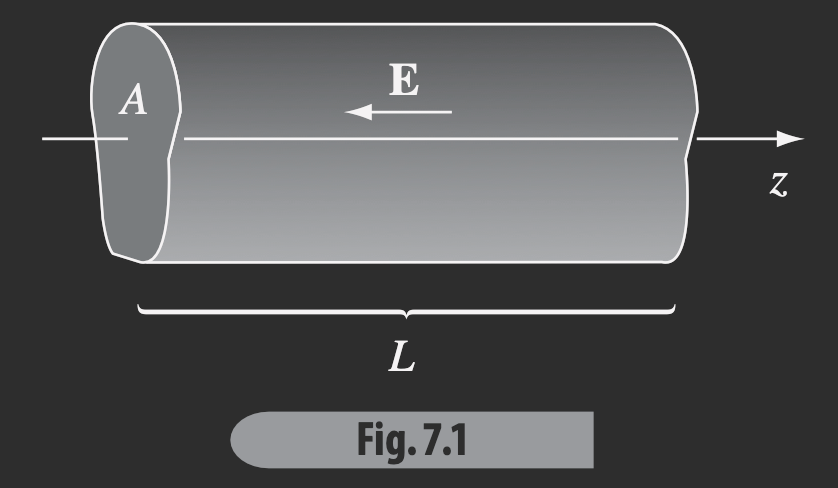
\includegraphics[width=0.5\linewidth]{fig7_1.png}
    \caption{Cylindrical Resistor}
    \label{fig:gr7_1}
\end{figure*}

The current $I$ flowing through the resistor is given by
\begin{align*}
    I = J A = \sigma E A = \sigma \frac{V}{L} A = \frac{\sigma A}{L} V
\end{align*}

\paragraph{Example} Coaxial cable with inner radius $a$, outer radius $b$,
separated by a material with conductivity $\sigma$:

\begin{figure*}[ht]
    \centering
    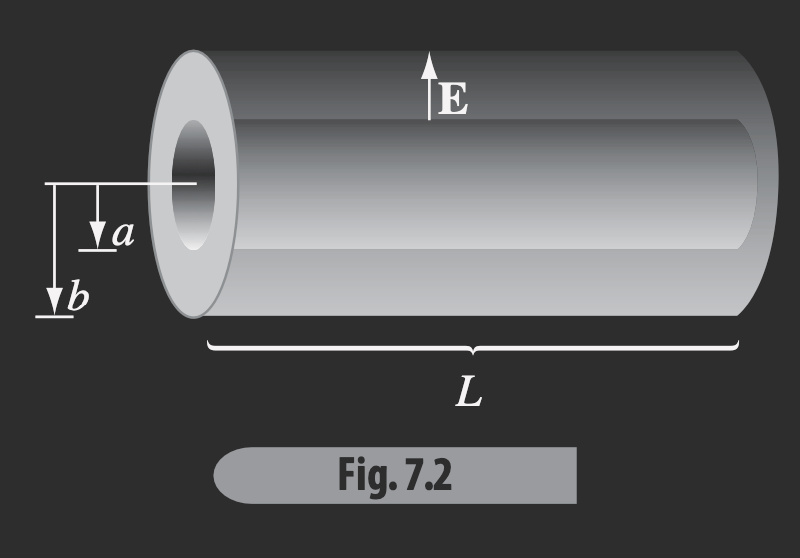
\includegraphics[width=0.5\linewidth]{fig7_2.png}
    \caption{Coaxial Cable}
    \label{fig:gr7_2}
\end{figure*}

The electric field will point radially outward in the region between the two cylinders:
\begin{align*}
    E = \frac{\lambda}{2\pi \epsilon_0 s} \vu s
\end{align*}
where $\lambda \sim$ charge/length. We get the current
\begin{align*}
    I = \int \vb J \cdot \dd{\vb a} = \sigma \int \vb E \cdot \dd{\vb a} = \frac{\sigma}{\epsilon_0} \lambda L
\end{align*}
and the potential
\begin{align*}
    V = -\int_b^a \vb E \cdot \dd{\vb l} = \frac{\lambda}{2\pi \epsilon_0} \ln \frac{b}{a}
\end{align*}
So we get
\begin{align*}
    \boxed{
        I = \frac{2\pi \sigma L}{\ln(b/a)} V 
    }
    \qquad \boxed{V = IR}
\end{align*}
which is the more common form of Ohm's Law.

For simple steady currents, we know that
\begin{align*}
    \div \vb J = 0
\end{align*}
$\to$ no source or sink of charge. Furthermore, from Ohm's law,
\begin{align*}
    = \div (\sigma \vb E) = \sigma \div \vb E = 0
\end{align*}
$\implies$ uniform $\vb E$ in conductors carrying steady currents.

So $\vb J = \sigma \vb E$ tells us a steady current flows due to an electric field, \emph{but}
$\vb F = q \vb E = m \vb a$ tells us that the electrons should accelerate\dots
Think of it like this: Electrons are like cars stopping at a stop sign;
they accelerate but then stop when they reach the next stop sign,
so they have a constant average velocity as they accelerate and stop.
This average is roughly
\begin{align*}
    v_\text{avg} = \frac{1}{2} a \tau = \frac{1}{2} \frac{a \lambda}{v_\text{thermal}} = \frac{1}{2} \frac{q E \lambda}{m v_\text{thermal}}
\end{align*}
so for $n$ moles per unit volume of charge and $f$ electrons per molecule
\begin{align*}
    \vb J = n fq v_\text{avg} = \qt(\frac{nf q^2 \lambda}{2m v_\text{thermal}}) \vb E
\end{align*}

How much energy/time is transferred to conductor?
\begin{align*}
    V \equiv \frac{W}{q}, \quad I \equiv \frac{q}{s} \implies P = IV = I^2 R
\end{align*}
aka the ``Joule heating law''.

\newpage
\subsubsection{Electromotive Force}

$\mathcal{E}$ or EMF

Current can experience forces
\begin{align*}
    \vb f = \vb f_s + \vb E
\end{align*}
where $\vb f$ is the total force/charge, and $\vb f_s$ can be chemical (from battery), mechanical (piezoelectric), etc.

The EMF can be the line integral
\begin{align*}
    \mathcal{E} = \oint \vb f \cdot \dd{\vb l} = \oint \vb f_s \cdot \dd{\vb l} + \cancel{\oint \vb E \cdot \dd{\vb l}}
\end{align*}
where the second terms cancels from Stokes's $\curl \vb E = 0$.
This EMF has units of volts, but it is not a potential difference....

% fig7_7.png
\begin{figure*}[ht]
    \centering
    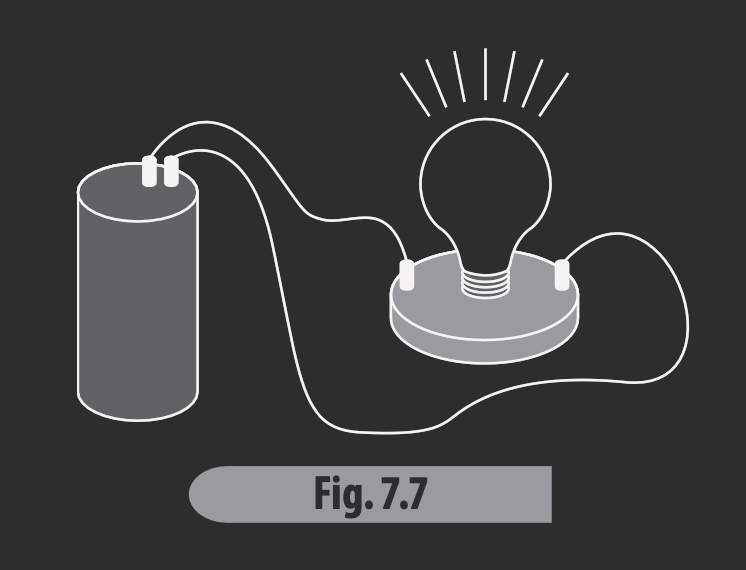
\includegraphics[width=0.5\linewidth]{fig7_7.png}
    \caption{EMF}
    \label{fig:gr7_7}
\end{figure*}
In the current wire connected to the battery (EMF), there is a $\sigma \sim 1/\rho \to R$ such that
$V = IR$ or in terms of the EMF $\mathcal{E} = IR$.
In the battery we idealize $\sigma \to \infty$ thus $R \to 0$. 

\subsubsection{Motional EMF}
``(E)motional'' 
\begin{figure*}[ht]
    \centering
    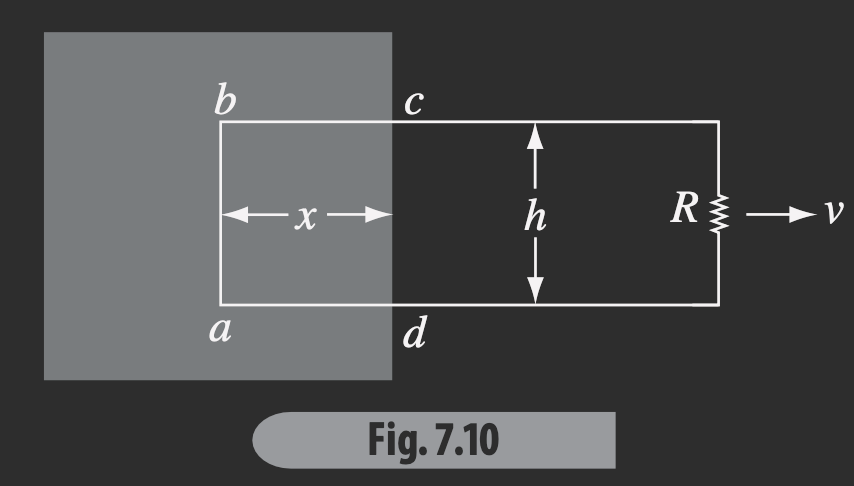
\includegraphics[width=0.5\linewidth]{fig7_10.png}
    \caption{Motional EMF}
    \label{fig:gr7_8}
\end{figure*}

For a B-field into the page, the current moves clockwise (RHR),
so the EMF is providing a magnetic force and not just a potential difference:
\begin{align*}
    \mathcal{E} = \oint \vb f_\text{mag} \cdot \dd{\vb l} = v B h = I R_\text{wire}
\end{align*}
We can also think of the area in the magnetic field as a flux
\begin{align*}
    \Phi = \int \vb B \cdot \dd{\vb a} = B h x = B \textrm{area}
\end{align*}
so the time rate of change (as we pull the wire with velocity $v$) is
\begin{align*}
    \dv{\Phi}{t} = B h \dv{x}{t} = -B h v
\end{align*}
or generally
\begin{align*}
    \mathcal{E} = -\dv{\Phi}{t}
\end{align*}
AKA ``Faraday's Law''.

\newpage
\lhead{Lecture 23: 11/19/24}
\subsection{Electromagnetic Induction}
\subsubsection{Faraday's Law}
$\sim 1831$ish Faraday observed three important experiments:
\begin{itemize}
    \item [1.] Moving a loop of wire rightward through a magnetic field induced a current in the wire.
    \item [2.] Moving a magnet to the left also induced a current.
    \item [3.] Increasing the magnetic field strength of a stationary magnet also induced a current on the
    stationary loop of wire.
\end{itemize}
(1.) Describes motional EMF, (2.) changes at rest! Empirically
\begin{align*}
    \mathcal{E} = \oint \vb E \vdot \dd{\vb l} = - \dv{\Phi}{t}, \quad \Phi = B A
\end{align*}
where $\Phi = \int_S \vb B(\vb r) \vdot \dd{\vb a}$ so
\begin{align*}
    \implies \oint \vb E \vdot \dd{\vb l} = \int_S (\curl \vb E) \vdot \dd{\vb a} = - \int_S \pdv{\vb B}{t} \vdot \dd{\vb a}
\end{align*}
which gives us Faraday's Law
\begin{align*}
    \boxed{
        \curl \vb E = -\pdv{\vb B}{t}
    }
\end{align*}

\subsubsection{The Induced Electric Field}
\begin{gather*}
    \curl E = 0 \to = -\pdv{\vb B}{t} \\
    \div \vb E = \frac{\rho}{\epsilon_0} \to = 0
\end{gather*}
Where we can get the magnetostatics equations by changing the terms
\begin{align*}
    \curl B = \mu_0 J, \qquad \div B = 0
\end{align*}
From the Biot-Savart Law,
\begin{align*}
    \vb E = -\frac{1}{4\pi} \int \frac{\pdv{\vb B}{t} \cross \vu \scriptr}{\scriptr^2} \dd{\tau} = -\frac{1}{4\pi} \pdv{t} \int \frac{\vb B (\vb r) \cross \vu \scriptr}{\scriptr^2} \dd{\tau}
\end{align*}
and using the Ampere's law integral form $\oint \vb B \vdot \dd{\vb l} = \mu_0 I_\text{enc}$, we have this integral form of Faraday's law
\begin{align*}
    \oint \vb E \vdot \dd{\vb l} = -\dv{\Phi}{t}
\end{align*}

\paragraph{Example} A uniform B-field $\vb B = B(t) \vu z$ filling a circular region of radius $s$.
When B changes, what is E?
\begin{align*}
    \oint \vb E \vdot \dd{\vb l} = E 2\pi s
\end{align*}
so
\begin{align*}
    = -\dv{\Phi}{t} = -\dv{t}[\pi s^2 B(t)] = -\pi s^2 \pdv{B}{t}
\end{align*}
Thus we have a circular electric field
\begin{align*}
    \vb E = -\frac{s}{2} \pdv{B}{t} \vu*\phi
\end{align*}

\paragraph{Example} Ring of radius $b$ with line charge $\lambda$ concentric with a region with magnetic field $\vb B = B_0 \vu z$,
but constrained to a region smaller than the ring $a$.

Again, an amperian loop of radius $s$ so
\begin{align*}
    \oint \vb E \vdot \dd{\vb l} = E 2\pi s = -\dv{\Phi}{t} = -\pi s^2 \pdv{B}{t} \implies \vb E = -\frac{s}{2} \pdv{B}{t} \vu*\phi
\end{align*}
inside the magnetic field region. Outside the magnetic field region, we have
\begin{align*}
    \oint \vb E \vdot \dd{\vb l} = E 2\pi s = -\pi a^2 \dot{\vb B} \implies \vb E = -\frac{a^2}{2s} \pdv{B}{t} \vu*\phi
\end{align*}
So at the ring or $s = b$,
\begin{align*}
    \vb E = -\frac{a^2}{2b} \pdv{B}{t} \vu*\phi
\end{align*}

The torque on the segment of the ring is 
\begin{align*}
    F = dq E
\end{align*}
so
\begin{align*}
    \dd \vb N = \vb r \cross \vb F = b \dd q E = b \lambda E \dd{l}
\end{align*}
The total toque is
\begin{align*}
    \vb N = b \lambda \qt(
        - \frac{a^2}{2b} \dot{B} \oint \dd{l} = - b \lambda \pi a^2 \dot{B} \vu*\phi
    )
\end{align*}
And the angular momentum is
\begin{align*}
    \int N dt = -\lambda \pi a^2 b \int_{B_0}^0 \dd{B}
\end{align*}
so
\begin{align*}
    \implies \Delta \textrm{ang momentum} = \lambda \pi a^2 b B_0
\end{align*}
\end{document}